\chapter{Methodology}
\label{chap:methodology}

This chapter describes the core stages of the proposed animal re-identification pipeline, used in both the classifcation mode and counting mode: preprocessing, feature extraction (global and local), aggregation of local descriptors into Fisher vectors (FV) and geometric verification used as an additional consistency check and for scoring.


\section{Preprocessing}
Wildlife images are rarely captured under controlled conditions, illumination can vary significantly, there can be backgroud clutter and/or occlusion. Preprocessing is used to reduce the variation and potential background bias.

\subsection{Mantiuk Tone Mapping}
Tone mapping compresses the dynamic range and enhances local contrast, making subtle patterns on the animal body more visible. Following the recommendation in \cite{springerSpeciesAgnosticPatterned}, this thesis uses Mantiuk tone mapping as an optional preprocessing step.

\subsection{Segmentation with Grounded SAM2}
Even if the images in a dataset are cropped, backgroud can still dominate local or global feature extraction which can lead to background bias. To eliminate this effect, a segmentation-based pipeline is used to isolate the animal from the background. The pipeline first localizes the animal using a text prompted dectector (GroundingDINO)\cite{groundingdino} and then produces a pixel level mask using Segment Anything Model 2 (SAM2)\cite{ravi2024sam2}. The mask is applied with soft edges to avoid introducing shart boundaries that could create non-existent keypoints.

\begin{figure}[H]
    \centering
    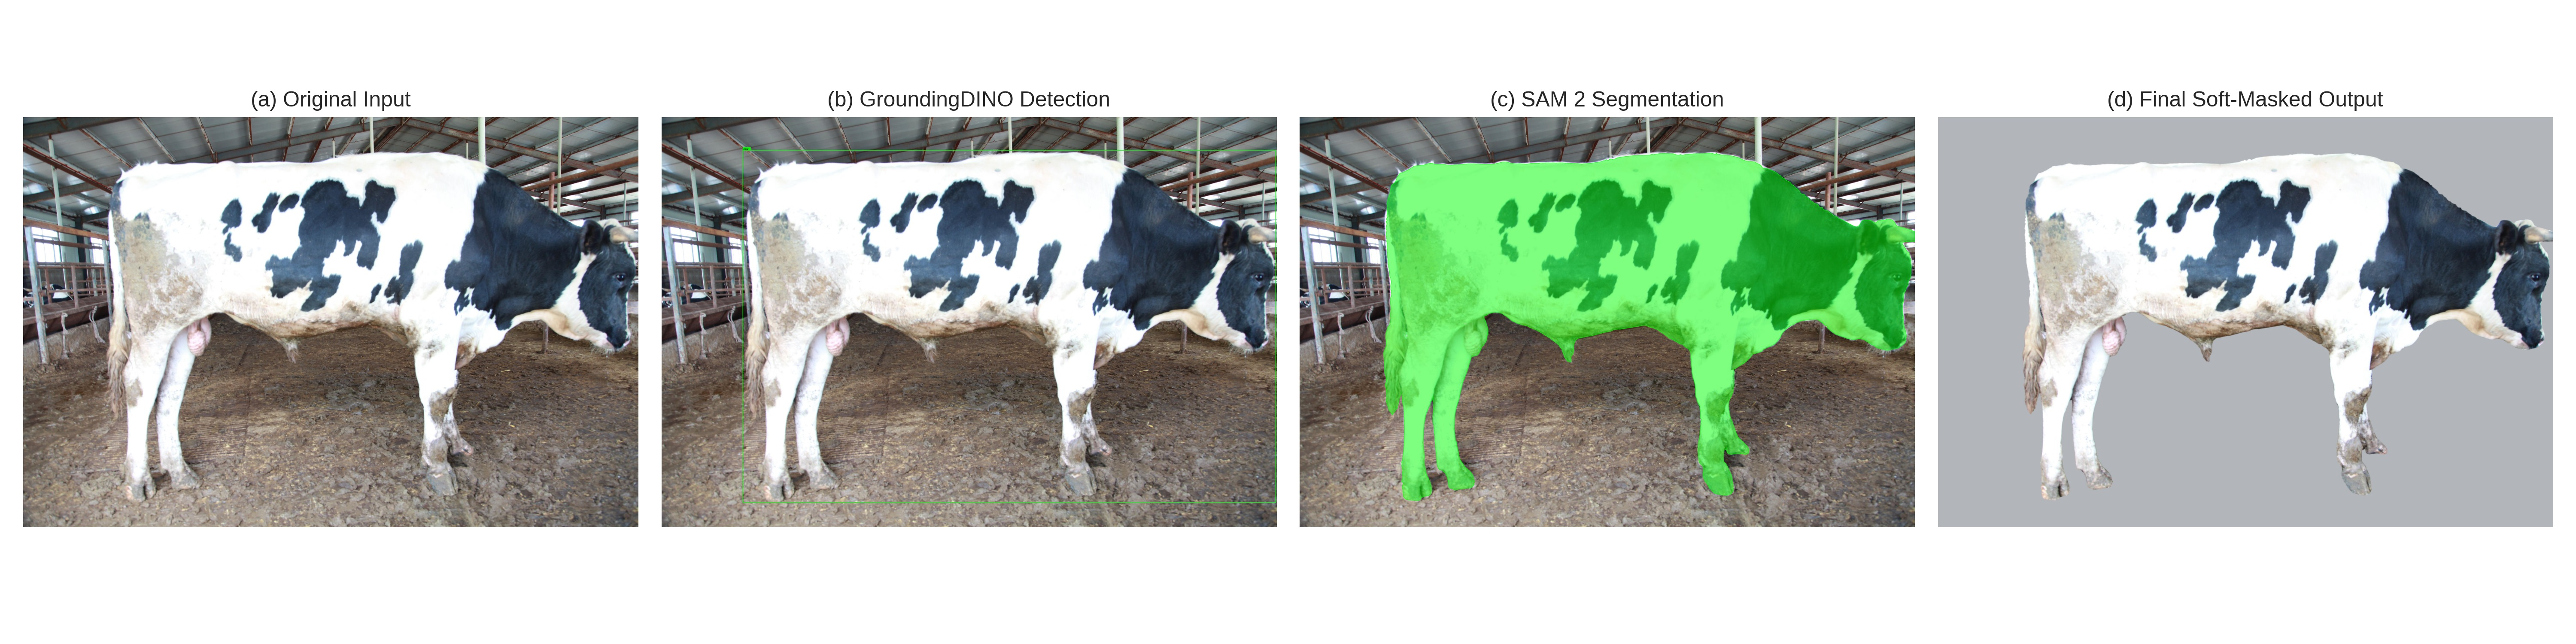
\includegraphics[width=0.95\linewidth]{Figures/segmentation_pipeline_vis.JPG}
    \caption{Overview of the segmentation-based preprocessing pipeline used for background removal.}
    \label{fig:segmentation_pipeline}
\end{figure}

Segmentation was not applied to all datasets in this thesis since some already came segmented or, in case of CTai, were already cropped so tightly that it was deemed unnecessary. 

\section{Feature Extraction}
\label{sec:feature_extraction}
Feature extraction is a critical component of animal Re-Identification pipelines, converting raw image data into a representation that can be compared across observations. This thesis uses two complementary families of features: global embeddings and local features.

\subsection{Why combine global and local features?}
Global embeddings summarize the entire image into a single vector and provide a fast, strong retrieval signal. Local features, on the other hand, represent an image as a set of keypoints and descriptors, which can capture fine-grained details and allow geometric consistency checks. These two feature families are evaluated both independently and in combination in later experiments.

\subsection{Global Embeddings}
\label{subsec:global_embeddings}

Global embeddings are a fixed-length feature vector produced by a pre-trained neural network (MD). Two images can then be compared by measuring the distance or similarity between their embeddings (in this thesis, cosine similarity is used).

For global embeddings, I used MegaDescriptor-L-384\cite{čermák2023wildlifedatasetsopensourcetoolkitanimal}, a large Swin Transformer model trained specifically for animal re-identification. It was trained on 29 publicly available datasets from WildlifeDatasets collection\cite{čermák2023wildlifedatasetsopensourcetoolkitanimal}. This provides a strong baseline similarity signal that is efficient and fast to compute and can be fused with the results of local methods.\cite{cermak2024wildfusionindividualanimalidentification}

\subsection{Local Features}
\label{subsec:local_feature_detection}
Local features model an image as a set of keypoints and associated descriptors. Matching local features between two images can give a similarity signal and also enables geometric verification. In practice, this is a two-step process: first keypoints are detected, and then each keypoint is described with a feature vector.

In this thesis, I used three modern learning-based local feature extractors:
SuperPoint\cite{DeTone2018SuperPoint}, DISK\cite{tyszkiewicz2020disklearninglocalfeatures},
and ALIKED\cite{zhao2023alikedlighterkeypointdescriptor}. Although each method performs
well individually, experiments showed that they are complementary, so they were also used
as an ensemble. These methods were selected because they work well out-of-the-box without
dataset-specific fine-tuning, while learning-based local features generally provide stronger
matching performance than classical handcrafted alternatives such as SIFT\cite{Lowe2004SIFT}.

Once keypoints are detected, we compute descriptors that summarize the appearance of the local region around each keypoint. An effective descriptor should be discriminative (distinguishing one region from another) and robust (invariant to geometric transformations).

\subsubsection{SuperPoint}
SuperPoint\cite{DeTone2018SuperPoint} uses a single convolutional network with two heads:
one predicts interest-point scores and the other predicts dense local descriptors.
It is trained in a self-supervised manner using synthetic homographic warps, which encourages
both detector repeatability and descriptor consistency under viewpoint changes.

\subsubsection{DISK}
DISK (DIScrete Keypoints)\cite{tyszkiewicz2020disklearninglocalfeatures} is an end-to-end
trainable framework that jointly learns keypoint detection and description. Its training
objective directly optimizes matching quality across image pairs, making it well suited for
retrieval and re-identification settings where reliable correspondence is required.

\subsubsection{ALIKED}
ALIKED\cite{zhao2023alikedlighterkeypointdescriptor} is a lightweight learned detector-descriptor
model designed for efficient local feature extraction. It uses a deformable transformation
strategy to better adapt to geometric variation while keeping inference computationally practical.
In this thesis, ALIKED provides a strong speed-accuracy trade-off and complements SuperPoint and
DISK in the ensemble setting.


\subsection{Local Matching}
Local descriptors are compared by matching keypoints between images. In this thesis, matching is performed with LightGlue\cite{lindenberger2023lightgluelocalfeaturematching}. Concretely, for each image pair LightGlue is provided with the extracted keypoint coordinates and their descriptors (from SuperPoint/DISK/ALIKED) and it outputs a set of tentative matches (index pairs of matching keypoints). We then use those matches as input to geometric verification (Section~\ref{sec:geometric_verification}).

\begin{figure}[H]
    \centering
    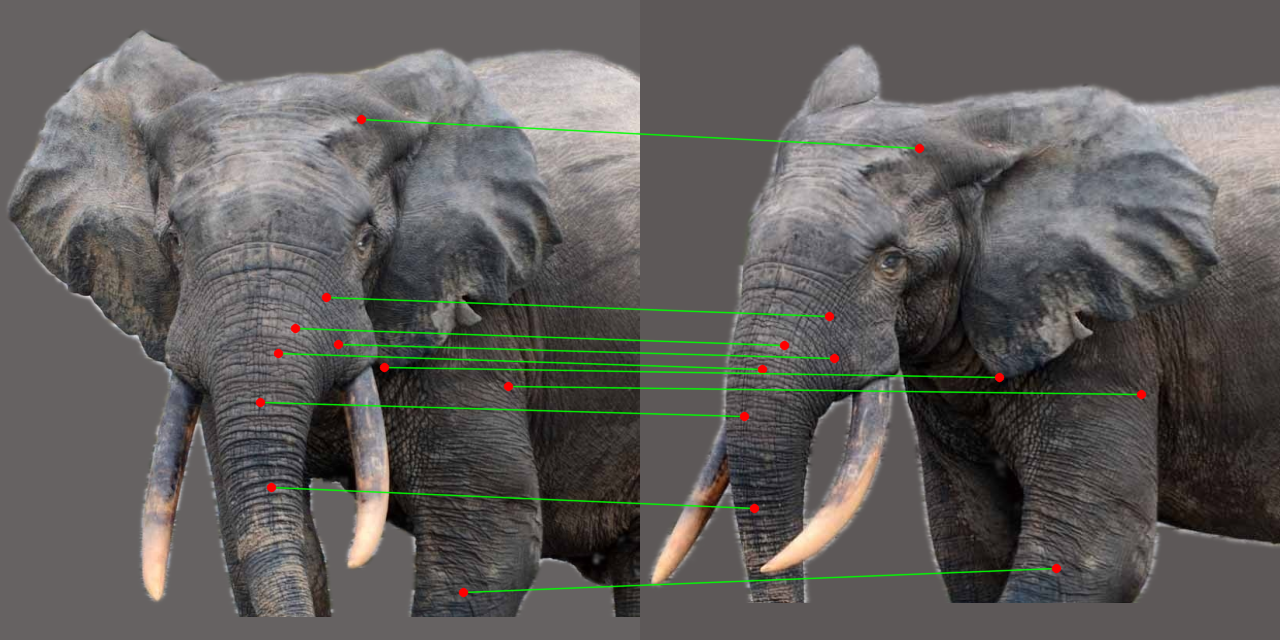
\includegraphics[width=0.95\linewidth]{Figures/visualize_matches.png}
    \caption{Example local feature matches between two images with backgrounds removed. Limited to 10 keypoints for visual clarity.}
    \label{fig:visualize_matches}
\end{figure}

\section{Feature Aggregation and Representation}
\label{sec:feature_aggregation}
Local feature matching is powerful but computationally expensive when comparing many query images against a large database. To enable efficient large-scale comparison, this thesis also aggregates sets of local descriptors into a single fixed-length representation using Fisher Vectors (FV)\cite{5540009}. The FV representation is built on PCA (Principal Component Analysis) for dimensionality reduction and GMM (Gaussian Mixture Model) that servers as a visual vocabulary\cite{springerSpeciesAgnosticPatterned}.


\subsection{Training PCA and GMM models}
\label{sec:pca_gmm_training}

Feature descriptors extracted from images can be high-dimensional and noisy. Thus, dimensionality reduction and normalization are performed to improve efficiency and accuracy.

Initially PCA is applied to decorrelate and reduce the dimensionality of the descriptors. PCA projects the original descriptors onto a lower-dimensional subspace defined by the principal eigenvectors of the covariance matrix computed from the descriptors. This is also important later on for the computation of fisher vectors because they produce very large descriptors.\cite{springerSpeciesAgnosticPatterned}

After dimensionality reduction, a Gaussian Mixture Model (GMM) is trained on the reduced descriptors. A GMM models the descriptor distribution as a weighted sum of $K$ Gaussian components, each parameterized by mean vectors $\{\mu_k\}$, covariance matrices $\{\Sigma_k\}$, and weights $\{\pi_k\}$. Specifically, a GMM is defined as:
\begin{equation}
    p(x) = \sum_{k=1}^{K}\pi_k \mathcal{N}(x|\mu_k,\Sigma_k),
\end{equation}

where $\mathcal{N}(x|\mu_k,\Sigma_k)$ denotes the probability density function of the $k$-th Gaussian component. This codebook (the trained GMM) captures the visual vocabulary and statistical distribution of the reduced descriptors from the training images.\cite{springerSpeciesAgnosticPatterned}

In simpler terms, PCA finds the directions in which the descriptor values vary the most and keeps only those, so each feature becomes a shorter, uncorrelated vector that is faster to store and compare. Then we model how these compact vectors are distributed. GMM model assumes that the whole set of vectors can be grouped into a number of smooth clusters, each cluster described by it's mean, spread and relative weight in the mixture. Together, these clusters form a codebook meaning that every new descriptor can be represented as a weighted combination of the nearest clusters, giving us both a compressed encoding and a way to compute similarity for matching or classification which is of crucial importance in re-identification task. 

\subsection{Fisher Vector Computation}
\label{sec:fisher_vector_computation}
Fisher vectors (FV) are an image representation technique that captures statistical deviations of local features from a visual vocabulary (codebook) modeled by GMM. FV measures how features differ from typical patterns in a reference GMM and they encode both first-order differences (mean shifts) and second-order differences (variance changes) in feature distribution. The output is a high-dimensional vector that acts as a "signature" of an image's unique feature distribution. Basically, given a set of descriptors extracted from a single image, FV encodes how these descriptors deviate from the trained GMM parameters. Fisher Vectors represent the gradients of the log-likelihood function with respect to the GMM parameters. Formally, given an image with descriptors $X = \{x_t\}_{t=1}^{T}$ where $\lambda$ is a vector of GMM parameters and $u_\lambda$ is a probability density function modeling the distribution of the data. 

This gradient is formally knows as the score function\cite{springerSpeciesAgnosticPatterned}. It measures the sensitivity of the log-likelihood to changes in the model parameters, essentially indicating how to adjust the GMM to better fit the observed features. 

\begin{equation}
G_\lambda^X = L_\lambda \log u_\lambda(X),
\end{equation}

When constructing a FV for an image, a set of local features is assumed to be independent which means that the final descriptor can be constructed as a sum of Fisher Vectors for each local feature:\cite{springerSpeciesAgnosticPatterned}

\begin{equation}
G{_\lambda^{X}} = \sum_{t = 1}^{T} L_{\lambda} \nabla_{\lambda} \log u_{\lambda}(x_t)
\end{equation}

The matrix $L_\lambda$ is derived from the Fisher Information Matrix and is used to "whiten" or to normalize the gradients\cite{article}, making them more discriminative and suitable for use in classification later on.

Following the standard practice, this vector is computed separately for means and variances, resulting in a final vector of dimension $2KD$, where $K$ is the number of Gaussian components and $D$ the dimensionality of the PCA-reduced descriptors. L2 and power normalization have also been applied since they have been shown\cite{10.1007/978-3-642-15561-1_11} to generally improve the performance of the method.

FV have also been chosen because they have been shown to perform better that bag-of-words approaches.\cite{5540009}

\subsection{Parameter Choices and Rationale}
\label{sec:parameter_choices}

Several key parameters influenced the effectiveness of Fisher Vectors for the re-identification task during the development:

\begin{itemize}
    \item \textbf{Number of PCA components ($N_{PCA}$):} A balance between dimensionality reduction and retention of discriminative information.
    \item \textbf{Number of GMM components ($N_{GMM}$):} Controls the granularity of the visual codebook. More components typically yield richer representations but increase computational complexity.
\end{itemize}

These parameters were empirically determined based on experimenting and computational constraints. Specifically, the PCA dimension was selected to retain approximately 95\% of descriptor variance. The number of GMM components was chosen to balance accuracy and computational efficiency. The best results were achieved, with $96$ PCA components, $256$ GMM components.

\section{Geometric Verification}
\label{sec:geometric_verification}
Geometric verification is used to make sure that matched keypoints between images truly correspond to the same physical locations on an animal reducing false positives that arise from visual similarites alone. This step is crucial in refining the initial matches obtained through descriptor-based feature matching by enforcing spatial consistency.\cite{springerSpeciesAgnosticPatterned}

\subsection{Theoretical Foundation}
Local feature descriptors such as DISK\cite{tyszkiewicz2020disklearninglocalfeatures} or KeyNet combined with AffNet and HardNet \cite{keynet, mishkin2018repeatabilityenoughlearningaffine, Mishchuk2017HardNet}, offer robust initial matches based on visual similarity. However, matches that are generated purely from descriptor similarity may include mistakes, especially in visually cluttered or repetitive environments common in wildlife images. Geometric verification, as suggested in \cite{springerSpeciesAgnosticPatterned}, addresses this by validating matches through spatial coherence checks. 

\subsection{Establishing Initial Correspondences}
Initial correspondences are established trough descriptor matching using LightGlue\cite{lindenberger2023lightgluelocalfeaturematching}, an attention-based method. Initially methods like Lowe's ratio test were considered but matching with LightGlue proved significantly faster and more accurate, effectively eliminating the need for traditional filtering methods.

\subsection{Transformation Estimation}
The core of GV involves estimating a homography transformation between matched keypoints using RANSAC (Random Sample Consensus). RANSAC iteratively samples minimal subsets of correspondences, computes candidate transformations and evaluates their agreement with the remaining matches. Matches that fall within a defined spatial threshold are considered inliers. 

\subsection{Scoring and Verification}
Matches are assessed primarily by their inlier count, the number of matches consistent with the estimated homography, and their spatial distribution:

    \begin{itemize}
        \item \textbf{Inlier count:} Number of correspondences that agree with the estimated transformation; higher counts suggest more reliable matches.
        \item \textbf{Inlier ration: } Normalizes the inlier count by the total number of tentative matches,
  $$
  r = \frac{|I|}{|C|},
  $$
  where $|I|$ denotes the inlier count and $|C|$ the total correspondences.
        \item \textbf{Combined scoring:} Integrates geometric consistency with descriptor similarity (fisher vector distances or global distances) to leverage both spatial and appearance information.
    \end{itemize}
Penalties for low inlier counts or poor geometric coherence discourage accepting borderline matches, improving the overall system reliability and accuracy.
